\section[h]{Formal Semantics}
\label{sect:semantics}

In this section we describe the formal semantics of some major language elements. In doing so we use a parametrized formal semantics, where the parameters govern the intervals at which the system is observed(\refsect{exec}) and how the system evolves with respect to time(\refsect{dynamics}). Essentially, we specify the semantics of the language, provided there is a procedure to compute the physical control component of a system. For instance, in the race application described in \refsect{Eg}, we parameterize the language semantics with the procedure for computing the positions of the robots at a given time. The event block is like the discrete step of a hybrid automaton, and the dynamic behavior is the continuous trajectory\cite{hioa}. The discrete part of the system corresponds to the programs, which interact with the physical environment using the \s{doReach} abstraction. The programs communicate with each other using shared variables.
\begin{center}
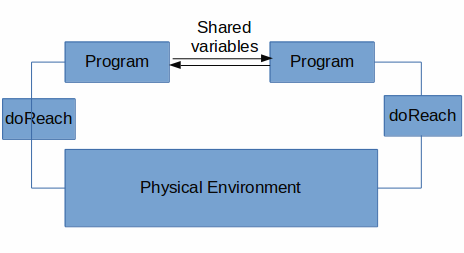
\includegraphics[scale=0.3]{struct.png}
\end{center}
We explain this further in the following sections, starting with a description of the system state. We then describe the major features of the language semantics, including the time model and the dynamics model, which parametrize the semantics. 
 
A system consists of \textbf{N} agents $A_1$, ..., $A_N$. In the implementation, we assume that this $N$ is known beforehand. In \refsect{syntax}, we described the structure of applications written in this language; each application is written in terms of events. We say that an event has occurred if its precondition was evaluated as true, and the corresponding effect was executed. Once an event has occurred, the program control goes back to the top of the event block. The event block (\s{eventBlock}) is said to be executed when any event in the event block occurs once. Given an agent running an application, its event block can be executed repeatedly while the application continues to run. Communication between agents takes place through shared memory updates. Shared memory updates require mutual exclusion, which is implemented by a locking mechanism. We describe the \verb|atomic| construct, which is used for mutual exclusion, in \refsect{locking}.


\subsection[h]{Configuration}
The configuration, or state, holds program variables, objects, and the execution context. We omit implementation minutiae, and only show relevant features. In the configuration, an agent is represented by an \s{agent} cell. Recall that a cell is a configuration unit, which is denoted by $\langle \mbox{cell-type} \rangle_{\mbox{cell-name}}$. For instance, a cell maintaining the \s{position} of an agent, which has type \verb|ItemPosition| will be represented as $\langle {\verb|ItemPosition|} \rangle_{\s{position}}$. Cells can also be composite cells, or containers of other cells. They will just be denoted by $\langle\mbox{cell-contents}\rangle_{\mbox{cell-name}}$.  

Each agent is represented by a composite cell, because the code is executed at agent level, and requires agent-specific information. An \s{agent} is identified by a unique identifier \s{id} (which is an integer). Its configuration contains the following cells. 
\begin{itemize}
 \item  \s{k} : Contains an agent's own application code. Each line in this cell is rewritten (possibly to empty) as the semantics is executed.
 \item \s{id} : Contains the agent's unique integer identifier. 
 \item \s{memory} : Contains a map from variables to addresses. 
 \item  \s{position} : The current position of the agent. Note that we only include the position cell in the current semantics because the applications we intend to write are in the domain of robotics. We can create cells to time-varying attributes of the agents as required.  
 \item  \s{counter} : The \s{counter} cell of each agent in the configuration maintains the number of times the event block of that agent has executed.
 \item \s{lockState} : Denotes whether or not the agent holds the requested lock. We discuss locking in \refsect{locking}. 
\end{itemize}
\begin{figure*}[ht]
\large
\centerfloat
  %
  \renewcommand{\dotCt}[1]{\scriptstyle\textit{#1}}
  \newcommand{\rid}{\scriptstyle\textit{ID}_{\sf robot}}
  \newcommand{\env}{\scriptstyle\textit{Var} \;\mapsto\; \textit{Address}}
  \newcommand{\store}{\scriptstyle\textit{Address} \;\mapsto\; \textit{Value}}
  %
$
\kall{system}{
  \begin{array}{@{}c@{}}
     \kall{k}{\dotCt{K}} \mathrel{}
      \kall{id}{\dotCt{Int}}\mathrel{}
      \kall{memory}{\dotCt{.Map}} \mathrel{}
      \kall{position}{\dotCt{ItemPosition}} \mathrel{}
      \kall{counter}{\dotCt{Int}} \mathrel{}
      \kall{lockState}{\terminal{idle}}
  \\ \mathrel{}
  \end{array}
}
$
  %
\caption{Agent Configuration}
\label{fig:agentconfig}
\end{figure*}

\normalsize

 Each agent's \s{memory} cell is a map from \emph{all} variables(of type \s{Id}, short for string identifier), to addresses(of type \s{Int}). Both global and local variables are included in this \s{memory}. This amounts to maintaining local copies of global variables, which are consistent across agents.  
 
The top level cell is called the \s{system cell}, which represents the distributed agent system. This cell contains the following cells:
\begin{itemize}
\item \s{agents} : This is a container cell for \s{agent} cells. It can contain as many such cells as the number of agents running the application, denoted by multiplicity "*". 
\item \s{gMemory} : This is the global memory, contains a map from all shared variables to addresses in the memory . 
\item \s{MMap} : Each variable of the application has an address in memory; we will presently discuss the scope of said memory. \s{MMap} stands for memory map, which is a map from addresses in the memory to actual values corresponding to the variables. 
\item  \s{time} : This is cell for maintaining time elapsed. 
\item \s{counterMap} : This cell maintains the map of agent \s{ids} to their \emph{counter} (\refsect{exec}) values. We explain what that refers to, in the next paragraph. 
\item  \s{lockQueue}: This cell is used to maintain the order in which the lock requests have been made.
\item \s{transitionState} : This cell stores whether the system is currently demonstrating dynamic behavior or not.  
\end{itemize}
\begin{figure*}[ht]
\large
\centerfloat
  %
  \renewcommand{\dotCt}[1]{\scriptstyle\textit{#1}}
  \newcommand{\rid}{\scriptstyle\textit{ID}_{\sf robot}}
  \newcommand{\env}{\scriptstyle\textit{Var} \;\mapsto\; \textit{Address}}
  \newcommand{\store}{\scriptstyle\textit{Address} \;\mapsto\; \textit{Value}}
  %
$
\kall{system}{
  \begin{array}{@{}c@{}}
  \kall{agents}{
  	agent*
  } \mathrel{}
  \\ \mathrel{}
  \kall{gMemory}{\dotCt{.Map}}\mathrel{}
  \kall{MMap}{\dotCt{.Map}} \mathrel{}\\ 
  \mathrel{} \kall{time}{\dotCt{Int}} \mathrel{}
   \kall{counterMap}{\dotCt{.Map}} \mathrel{}
  \kall{lockQueue}{\dotCt{.List}} \mathrel{} \\
  \kall{transitionState}{\terminal{discrete}}\mathrel{}
  \\ \mathrel{}
  \end{array}
}
$
  %
\caption{System configuration.}
\label{fig:highlevelconfig}
\end{figure*}

\normalsize


\subsection[h]{Local Variable Declaration}
We first provide the semantic rules for processing variable declarations, as an introduction to reading the semantic rules in \K. When a local variable declaration is encountered while an agent's code is being processed, an entry is created in the \s{memory} cell, which maps the variable to the next available address in the \s{MMap}. A corresponding entry is created in the \s{MMap}, which maps the aforementioned address to an \s{undefined} value of the declaration type if the declaration is uninitialized. It maps to the value the variable was assigned otherwise. We now define the rule for local variable assignment.
\paragraph{Variable declaration rule: } The \s{k} cell of an agent holds the code being interpreted. Suppose we encounter a local variable declaration \s{T X;} where \s{T} is the type, and \s{X} is the name of the variable.  We use the ellipses to represent the fact that (possibly empty) contents of the cell after the element being rewritten do not matter. The variable declaration rule first rewrites the line of code to empty($\dotCt{}$). At the same time, it creates an entry in the \s{memory} cell which maps \verb|X| to \s{L}, where \s{L} is the next available address in the \s{MMap}. Creating an entry in the map is the same as rewriting an empty element to the entry at the end of the map, hence the rewrite rule has the form $\reduce{\dotCt{}}{{M}}$, where $M$ is the entry being created.

We omit the details of how we determine $L$, as it is not relevant. The rule also creates an entry in \s{MMap} with \s{L} corresponding to \s{undefined(T)} (undefined value of type \s{T}).  

\begin{figure*}[ht]
\krule[variable declaration]{
\kmiddle{agent}{
\kprefix{k}{
 \reduce{{\variable[type]T \variable[ID]X;}}{{}{\dotCt{}}} }
 \ksuffix{memory}{ \reduce{{\dotCt{}}}{{}{X \mapsto L}}}
}
\ksuffix{MMap}{
 \reduce{\dotCt{}}{{}{L\mapsto undefined(T)}
}}
}
{}{}{}{}
\krule[variable declaration with assignment]{
\kmiddle{agent}{
\kprefix{k}{
 \reduce{{\variable[type]T \variable[ID]X = V;}}{{}{\dotCt{}}} }
 \ksuffix{memory}{ \reduce{{\dotCt{}}}{{}{X \mapsto L}}}
}
\ksuffix{MMap}{
 \reduce{\dotCt{}}{{}{L\mapsto V}
}}
}
{}{}{}{}
\end{figure*}

It should be mentioned that we assume unbounded memory for simplifying the semantics specification.  

\subsection[h]{Time Advance Semantics}
\label{sect:exec}


While designing the current semantics of this language we assume that we are able to maintain a global clock (the \s{time} cell). The dynamic behavior of each agent in the system is time varying. Since global time is a part of the system configuration or state, we need to supply rewrite rules for advancing time.

 Recall that the event block describes the discrete behavior of each agent. We can say that event block execution takes zero logical time. An event block can execute numerous times between time rewrites. We now define the time model for this semantics. The time model $\tau$ is defined as a tuple $\tau = (\delta, n_0)$ where 
 \begin{itemize}
 \item $\delta$ : is the global time increment. 
 \item $n_0$ : is the number of times that the event block of each agent must execute before global time is advanced. We use the \s{counter} and \s{counterMap} cells in the configuration for bookkeeping about this parameter. 
 \end{itemize}
We can now provide the rules of time progression in our semantics, given a time model $\tau = (\delta,n_0)$. 

\paragraph{Counter Advance Transition:}
We first discuss how to increment the \s{counter} of an agent when it executes an event block once. To ensure that, as soon as the precondition of the event evaluates to true, the rest of the event block should be rewritten to empty. That means, given an event block \s{pre(C); eff : S Es} where \s{C} is a condition evaluating to true, \s{S} is the list of statements in the effect of that event, \s{Es} is the list of events following that; this event block rewrites to \s{S}. If \s{C} evaluates to false, this block rewrites to \s{Es}. We skip the details of the rewrite rules involved in this process. 
\s{endEventBlock} is a terminal that we introduce (using a rewrite rule) at the end of the event block. If while executing the semantics, an \s{endEventBlock} is encountered in the \s{k} cell, it should imply that an event has occurred, the \s{counter} should be incremented and  the event block should start executing from the top again.
 
 Consider an agent with \s{id} $i$. If an \s{endEventBlock} is encountered in its \s{k} cell, there is nothing more to do in the current execution. Given further, that the \s{count} cell value of the agent is $N$, the \s{k} cell is rewritten to empty. The \s{counter} cell is rewritten to $N+1$, and the corresponding value of its counter in the \s{counterMap} cell is also rewritten to $N+1$. This transition is enabled only as long as $N$ is less than $n_0$. This ensures that each agent executes its event block exactly $n_0$ times before the time increments. 
\vspace{-1mm}

\begin{figure*}[ht]
\krule[counter advance transition]{
\kall{agent}{
\begin{array}{@{}c@{}}
\kall{k}{
 \reduce{\terminal{endEventBlock}}{{\dotCt{}}}
}
\kall{id}{\variable[Int]i}
\kall{counter}{ \reduce{\variable[Int]{N}}{{{{\variable[Int]{N}}
  \mathrel{+_{\scriptstyle\it Int}}
  {{}\variable[Int]1}}}}}
\end{array}
}
\begin{array}{@{}c@{}}
\kmiddle{counterMap}{ \reduce{\variable[Int]{i}\mapsto N}{{{{{\variable[Int]{i}\mapsto \variable[Int]{N}+_{Int} 1}}}}}}
  \end{array}
}
{
  {{\variable[Int]{N}}
  \mathrel{<_{\scriptstyle\it Int}}
  {{}\variable[Int]n_0}}
}{}{}{}
\end{figure*}

Note that when the \s{endEventBlock} is encountered, we rewrite the entire \s{k} cell to empty. How does the next iteration of the event block start then? We maintain a copy of the original application code in the state information, which is copied into the \s{k} cell at the beginning of every iteration of the event block. We have not shown this (along with other implementation details) in the interest of clarity of expression. 
\paragraph{Time Advance Transition:}
Suppose that the \s{counterMap} cell, which maintains a map of ids to counter values of all agents, is $CM$. \s{findMax} and \s{findMin} are functions for computing the maximum and minimum in the range of a map respectively. If both the minimum and maximum values are equal, then all values in the range of the map are equal.  The \s{time advance} transition says that, given that the current global time is $T$, if all the counter values in $CM$ are equal to $n_0$, the global time is rewritten to $T+\delta$. The \s{transitionState} is set to \verb|dynamic| from \verb|discrete|. We do not show the rest of the configuration items because they do not appear in the condition or change with the time progression rule. 
\begin{figure*}[ht]

\end{figure*}
. 
\vspace{-4mm}
It is worth mentioning that while we designed the time progression such that the event block executes exactly $n_0$ number of times for each agent, we can easily change the design to accommodate different values for different agents. To do that, we modify the time model by adding another parameter $\rho$ to it. $\rho$ is a map from agent \s{ids} to integers. Instead of incrementing the counter by one every time an event occurs, agent with it $i$ increments its counter by $\rho[i]$. The number of times its event block executes is then $\floor{\frac{n_0}{\rho[i]}}$.


\section[h]{Locking}
\label{sect:locking}
We provide global locks to implement mutual exclusion for the atomic construct. 
	These locks have two major properties:
    \begin{itemize}
\item At any time, at most one agent can hold a lock. 
\item A agent needs to request a lock at most once before being eventually granted the lock. 
\end{itemize}
The first property ensures mutual exclusion and the second ensures that high frequency agents do not monopolize the lock. 
While defining the semantics it is easier for us to present the rules in terms of a single global lock on all multi-writer shared variables. This means that whenever an agent requests a lock it obtains a lock on all shared variables declared in the \verb|MW| block. Each agent has a cell called \s{lockState}, which is set to \s{idle} if the agent is not requesting or holding the lock, \s{request} if the agent has requested the lock but not been granted it yet, and \s{lock} if the agent is currently holding the lock. We maintain the lock queue or the order in which requests to the lock were made by agents, in the cell \s{lockQueue}. 

When an agent requests a lock, its \s{id} is added at the end of the \s{lockQueue} An agent which has requested a lock, is granted it if it is the first in the lock queue. Once an agent has requested a lock, its \s{lockState} is updated to \s{request}. An agent is not allowed to add itself to the \s{lockQueue} unless its \s{lockState} is \s{idle}. When the agent is at the beginning of the \s{lockQueue} and its \s{lockState} is \s{request}, then it can execute its atomic block. Once it has done so, it updates its \s{lockState} to \s{idle} again, and removes itself from the \s{lockQueue}. 

An agent is in the process of executing the effect of an event whose precondition evaluated to true, when it might need to request a lock. It is however, not allowed to execute the next line of code until it is granted the lock and can proceed. We force the \s{counter} to be incremented every time the agent checks its position in the \s{lockQueue}. The reason for this is to capture behavior where the lock may not be granted immediately. From our discussion in the previous section, the event block execution takes zero logical time. If the counters were not incremented while the agents were requesting a lock, all locks would be granted before \s{time} was incremented from the current value. This would then imply that all locks are granted while zero logical time passed, which is unrealistic behavior. We provide the rewrite rules governing locking below, again, given a time model $\tau = (\delta,n_0)$. 

\paragraph{Lock Request Transition:} The \s{lock request} transition is enabled when an agent with \s{id} \s{i}, encounters an atomic block containing statements \s{Ss}, when its \s{lockstate} is \s{idle}. Then, the agent adds a terminal \s{atomicEnd} just after the atomic block, to ensure that the agent releases the lock after executing it. At the same time, the agent adds itself to the end of the lock queue. The ellipses represent the fact that the lock queue may or may not be empty, it doesn't affect the application of the current rule. Again, we omit showing the irrelevant cells in this rule. 
\begin{center}
\begin{figure}
\label{fig:lock1}
\krule[lock request transition]{
\kprefix{agent}{
\begin{array}{@{}c@{}}
\kprefix{k}{\terminal{atomic :}\variable[Statement]Ss
 \reduce{\dotCt{}}{{\terminal{atomicEnd}}}
}
\kall{id}{\variable[Int]{i}}
\kall{lockState}{
 \reduce{\constant[\#Type]{idle}}{\constant[\#Type]{request}}
}

\end{array}
}
\ksuffix{lockQueue}{
{
 \reduce{\dotCt{}}{{\variable[Int]{i}}}
}}
}{}{}{}{}


\end{figure}
\end{center}
\paragraph{Atomic Wait Transition:} As indicated in above, we capture the fact that locks may not be granted immediately by enabling counter increment transitions when the \s{lockState} is \s{request} and the agent \s{id} is not at the head of the \s{lockQueue}. The rewrite rules in the semantics can fire whenever they are enabled, which means that this might result in an agent just continually incrementing its counter, and never doing anything else; thus simulating a failed or crashed agent. Since failure is only observed when communication fails, it can be assumed that the agent failed when it itself fails to communicate. 
\begin{figure}
\label{fig:lock}
\krule[atomic wait transition]{
\kmiddle{agent}{
\begin{array}{@{}c@{}}
\kall{id}{\variable[Int]{i_1}}
\kall{lockState}{
 {\constant[\#Type]{request}}
}
\kall{counter}{
\reduce{\variable[Int]N}{\variable[int]N{+_{\scriptstyle\it Int}} \constant[Int]1}
}
\end{array}
}
\kprefix{lockQueue}{\variable[Int]i_2}
\begin{array}{@{}c@{}}
\kmiddle{counterMap}{ \reduce{\variable[Int]{i}\mapsto N}{{{{{\variable[Int]{i}\mapsto \variable[Int]{N}+_{Int} 1}}}}}}
  \end{array}
}
{\variable[Int]i_1 !=_{\scriptstyle\it Int} i_2 \terminal{and} \variable[Int]N <_{\scriptstyle\it Int} \variable[Int]n_0 }{}{}{}
\end{figure}

\paragraph{Atomic Execution Transition:} The agent aquires the lock when it is at the beginning of the \s{lockQueue} and starts processing the statements inside the atomic block. The \s{counter} does not increase in this rewrite, because once the lock has been acquired, the agent can immediately execute the atomic block. 
\begin{figure}
\label{fig:lock}
\krule[atomic execution transition]{
\kprefix{agent}{
\begin{array}{@{}c@{}}
\kprefix{k}{
 \reduce{\terminal{atomic :}\variable[Statement]Ss}{{\variable[Statement]{Ss}}}
}
\kall{id}{\variable[Int]{i}}
\kall{lockState}{
 \reduce{\constant[\#Type]{request}}{\constant[\#Type]{lock}}
}

\end{array}
}
\kprefix{lockQueue}{\variable[Int]i}
\mathrel{}
}
{}{}{}{}
\end{figure}

\paragraph{Lock Release Transition}
Once the atomic block has been executed, the lock must be released, the agent must take itself out of the \s{lockQueue}, and set its own \s{lockState} to \s{idle}. The rest of the event continues to execute. Recall that in the lock request transition, we added a terminal \s{atomicEnd} after the atomic block. We can now use that to identify where the atomic block ends. 
\begin{figure}
\label{fig:lock}
\krule[lock release transition]{
\kprefix{agent}{
\begin{array}{@{}c@{}}
\kprefix{k}{
 \reduce{\terminal{atomicEnd }}{\dotCt{}}
}
\kall{id}{\variable[Int]{i}}
\kall{lockState}{
 \reduce{\terminal{lock}}{\terminal{idle}}
}

\end{array}
}
\kprefix{lockQueue}{\reduce{\variable[Int]i}{\dotCt{}}}
\mathrel{}
}
{}{}{}{}
\end{figure}
%\subsection{Dynamics}
\label{sect:dynamics}
We first present the semantic rules involving the \s{doReach} abstraction. 

\paragraph{doReach transition}
The \s{doReach} component interfaces with the application using flags \s{doReach\_done} and \s{doReach\_fail}. When \s{doReach} is invoked, the blackbox containing the implementation of \s{doReach} is called. Recall that \s{doReach} takes two arguments, the \emph{target}, and the \emph{obstacle}. The exact format of the obstacle is irrelevant to the semantics, as it is used by implementation specific objects in the \s{doReach} blackbox. \s{doReach} is technically invoked at each time increment. The target and the obstacles are set to current position and empty initially, unless the application specifies otherwise. Again, we omit the details of how we store these in the configuration. We now provide the rule to process the \s{doReach} statement when it appears in the application. 


\paragraph{doReach update transition: }When a \s{doReach} statement is encountered in the program, the statement itself is rewritten to empty. The $\curvearrowright$ is used to break down the program, which is seen as a single task, into a sequence of tasks. Therefore, it means after rewriting the \s{doReach} to empty, the \s{doReach} flags should be reset(\s{doReach\_done,doReach\_fail} are both set to false), which should in turn be followed by setting the target of this agent, and the list of obstacles. The \s{setTargetObs} function sets the values of target, obstacle , and current time. 
\begin{figure}
\label{fig:lock1}
\krule[doreach update transition]{
\kprefix{agent}{
\begin{array}{@{}c@{}}
\kprefix{k}{
 \reduce{\dotCt{\terminal{doReach} (T,O)}}{{\dotCt{}}} \curvearrowright resetFlags(i) \curvearrowright setTargetObs(T,O,T_0,i)
} 
\kall{id}{\variable[Int]{i}}\mathrel{}
\end{array}
}
\kall{time}{T_0}
}{}{}{}{}
\end{figure}
\vspace{-2mm}
\paragraph{doReach invoke transition} Recall that the \s{transitionState} cell of the system is set to \s{dynamic} when all the \s{counter} values of all agents reach $n_0$. Suppose the current \s{time} is $T_0$ The time advances by $\delta$. We then invoke the blackbox \s{doReachBB} to compute the new contents of the \s{position} cell of each agent at time $T_0 +\delta$, given that the position of the agent at time $T_0$ was $P$, the target \s{ItemPosition} is $T$, obstacles were stored in $O$, and the time increment was $\delta$. We omit the details of maintaining $T_0$, $O$ and $T$.
\begin{figure}
\label{fig:lock1}
\krule[doreach invoke transition]{
\kprefix{agent}{
\begin{array}{@{}c@{}}
\kall{id}{\variable[Int]{i}}
\kall{counter}{\reduce{N}{0}}
\kall{position}{\reduce{\variable[ItemPosition]P}{P_{1}}}
\end{array}
}\mathrel{}
\kmiddle{counterMap}{\reduce{i\mapsto N}{i \mapsto 0}}
\kall{transitionState}{dynamic}}
{N \mathrel{==_{\scriptstyle\it Int}} n_0 \terminal{and} P_{1} = \terminal{doReachBB}(P,T,O,T_0,\delta,i)}{}{}{}
\end{figure}


